% alt + shift + 1
% make projname.pdf
% wordcount: detex writeup.tex | wc -w

\documentclass[12pt]{article}
%------------------------Dimensions----------------------------

\topmargin=0.0in
\oddsidemargin=0.0in           % 1in margins at left and right
\evensidemargin=0in
\textwidth=6.5in               % US paper is 8.5in wide
\marginparwidth=0.5in

\headheight=0pt                % 1in margins at top and bottom
\headsep=0pt
\topmargin=0in
\textheight=9.0in              % US paper is 11.0in high

%adjustments...
\addtolength{\topmargin}{-0.5in}
\addtolength{\textheight}{1.0in}
\addtolength{\textwidth}{0.5in}
\addtolength{\oddsidemargin}{-0.25in}
\addtolength{\evensidemargin}{-0.25in}
                       
\pagestyle{empty}

%------------------------Packages----------------------------
\usepackage{textcomp}
\usepackage{longtable}
\usepackage{setspace}
\usepackage{amsmath,amssymb,amsthm}
\usepackage{graphicx}
\usepackage{epsfig}
\usepackage{subfig}
\usepackage[paperwidth=8.5in,paperheight=11in,margin=0.98in]{geometry}
\usepackage{listings,float}
\usepackage{color}
\usepackage{array}
\usepackage{cancel}

%------------------------Commands----------------------------
\newcommand{\be}{\begin{enumerate}}
\newcommand{\ee}{\end{enumerate}}
\newcommand{\bi}{\begin{itemize}}
\newcommand{\ei}{\end{itemize}}
\newcommand{\bv} {{\bf v}}
\newcommand{\bD} {{\bf D}}

\definecolor{listinggray}{gray}{0.9}
\definecolor{lbcolor}{rgb}{0.9,0.9,0.9}
\lstset{
	tabsize=4,
	rulecolor=,
	language=matlab,
	keywords={break,case,catch,continue,else,elseif,end,for,function,
      global,if,otherwise,persistent,return,switch,try,while},
        basicstyle=\footnotesize\ttfamily,
        upquote=true,
        aboveskip={1.5\baselineskip},
        columns=fixed,
        showstringspaces=false,
        extendedchars=true,
        breaklines=true,
        prebreak = \raisebox{0ex}[0ex][0ex]{\ensuremath{\hookleftarrow}},
        frame=single,
        showtabs=false,
        showspaces=false,
        showstringspaces=false,
        identifierstyle=\ttfamily,
        keywordstyle=\color[rgb]{0,0,1},
        commentstyle=\color[rgb]{0.133,0.545,0.133},
        stringstyle=\color[rgb]{0.627,0.126,0.941},
}

\captionsetup{width=.75\textwidth} 

\begin{document}
\pagestyle{plain} %pagenumbers
\title{CSCI 4/5576: The Random Logistic Map}
\date{December 17, 2014}
\author{Amy Le (5576)\\Long Tat (4576)\\Emily Bertelson (4576)\\Kristina Entzel (4576)}
\maketitle
\section{Abstract}
The purpose of this project is to characterize the Random Logistic
Map. In particular, we will be studying the stability of the map,
which includes locating fixed points and generating bifurcation
diagrams. The two main goals are:
\be
\item Find the expected number of order $p$ periodic orbits for a
  the random map ($p = 1, 2, 3, ...$)
\be
\item For an initial starting value $x_0 \in [0,1]$ and a specific
  random function $R_0(x)$, iterate until you
  find the fixed point(s), $x_i^*$ associated with $R_0(x)$. 
\item Classify the fixed points in terms of a period $p$ orbit. 
\item Each processor should take a different initial $x_0$ and report
  whether the initial condition led to finding a unique stable orbit  
\bi
\item The processors should be properly load balanced.
\item As each processor finishes its work, it will write its results
  to an HDF5 file (parallel i/o)
\ei
\item Repeat the above steps for a large number of different random
  maps $R_i(x)$, $i = 0, 1, 2,... \bar{N}$ in order to find the expected
  number of order $p$ periodic orbits for the random map.
\ee
\item Create a set valued bifurcation diagram \cite{lamb}
\be
\item For many values of $r \in [0,4]
$, and a fixed random function
  $R_0(x)$, plot the locations of the periodic orbits as a function of
  $r$. A period $p$ orbit will have $p$ corresponding $x$ values as
  its orbit locations (e.g. a period 1 orbit will have 1 fixed point,
  a period 2 orbit will have 2 fixed points, and so on). 
\bi
\item Read data from HDF5 file
\ei
\ee
\ee
As the map has an element of randomness to it, many
simulations (a large $\bar{N}$) would be required for statistical analysis. This project is a subset of a larger work in progress
and requires optimization. A serial implementation has been developed
in MATLAB. The parallel implementation will be in C++.
\section{Introduction}
The following equation is the fixed point iteration that the code
completes, where $R(x)$ is calculated by manipulating a random number generator.
\begin{equation}\label{randmap}
x_{n+1} = R(x_n)x_n(1-x_n)
\end{equation}
The exact details of how to calculate $R(x)$ are outlined below.
\begin{align*}
\begin{split}
\ln(R(x)) &= \xi(x)\\
\xi(x) &= \ln(r) + 2\sum^N_{n=1}a_n\cos(2\pi nx)-b_n\sin(2\pi nx)\\
a_n,b_n &\sim Unif(-M_n,M_n)\\
M_n &= \sqrt{1.5S_n}\\
S_n &= \alpha e^{-L|n|}\\
\alpha &= \sigma^2 \tanh(L/2)\\
\sigma &< \ln(4/r)\frac{\tanh(L/4)}{\sqrt{1.5\tanh(L/2)}}
\end{split}
\end{align*}
Where $L \in (0,1)$ represents the correlation length (and is fixed
for each simulation) and $r \in [0,4]$ is also fixed for each
simulation. Optimizations implemented in the code conversion:
\bi
\item Preferential use of the  multiply and add operators where possible, since
they less expensive than subtract and divide operators
\item I used a reduction on the loop that computes the Fourier Series
  in order to take advantage of the data parallelism with SIMD
\item Loop structure was reorganized to take advantage of C++ being row-oriented
\item I used inlining in the C++ code to reduce the number of function calls
\item The lack of a built in uniform random number generator that generates a random
double between two doubles made me create a psudeo random number
implementation with the use of \texttt{rand} and \texttt{srand}.
\lstinputlisting{rand_ex.m}
\ei


\begin{figure}[H]
	\begin{center}
		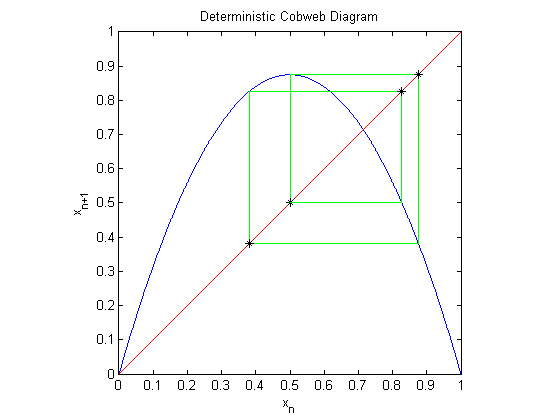
\includegraphics[scale=0.7]{det_cobweb}
\caption{nonrandom case}
	\end{center}
\end{figure}

\begin{figure}[H]
	\begin{center}
		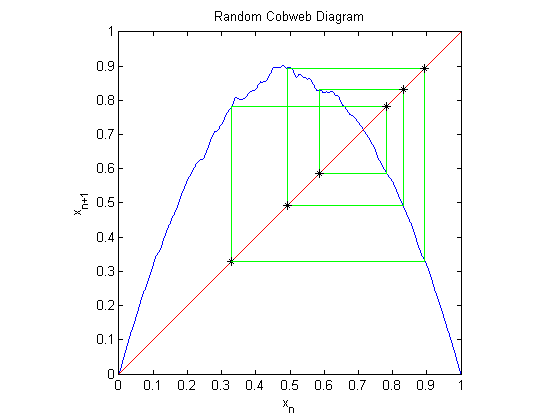
\includegraphics[scale=0.7]{rand_cobweb}
\caption{One instance of a random logistic map. This is a preliminary result from the serial implementation.}
	\end{center}
\end{figure}

\section{Method}
The general progression of the project is outlined below:
\be
\item Convert the Matlab code to C++ (object oriented)
\item Confirm the C++ versions of the code that we each produce work
  together correctly
\item Parallelize the C++ code
\bi
\item Use MPI to parallelize the mathematical computation
\item Invoke the load balancer to assign an initial condition to each
  fixed point iteration \cite{dlb}
\ei
\item Benchmark 
\bi
\item strong scaling study (speedup and efficiency)
\item weak scaling study (speedup and efficiency)
\ei
\ee
\noindent The table below summarizes how we have subdivided the project among
ourselves. 
\begin {table}[H]
\centering
\caption{Division of Labor}
    \begin{tabular}{ |p{1cm}|p{10cm}|} 
    \hline
    Amy &  make a random number distribution and use the cobweb
    diagram (fixed point) routine to return a list of subsequent iterations\\ \hline
    Long & calculate period order, given a list of subsequent iterations  \\ \hline
    Kristi & calculate the average number of period $p$ orbits, given
    a list of period locations, period orders, and starting positions\\ \hline
    Emily  & create the HDF5 file hierarchy to organize the simulation
    data; use links in the file to generate views of the data for easy
    plotting\\ \hline
    \end{tabular}
\end{table}

\subsection{Load Balancer}
\begin{figure}[H]
	\begin{center}
		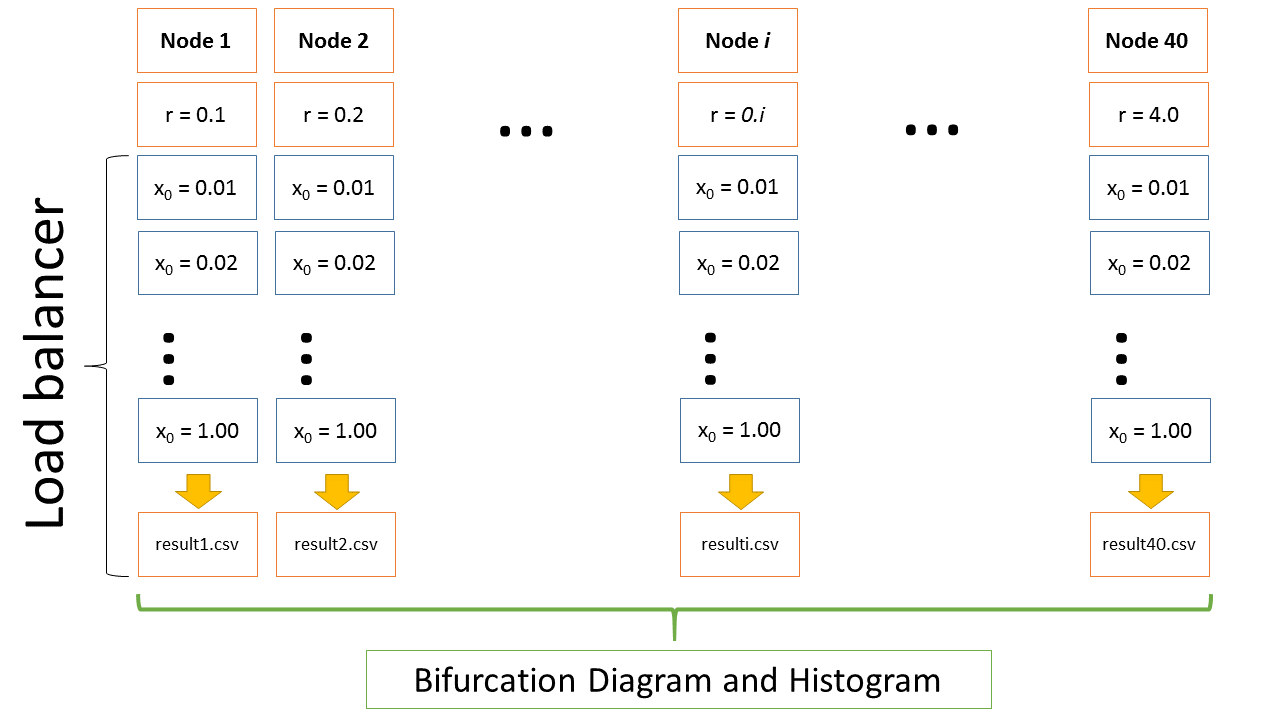
\includegraphics[scale=0.4]{load_balancer}
\caption{Load balancer.}
	\end{center}
\end{figure}

\subsection{HDF5}
A structure for the file has been devised:
\begin{tabbing}
	\hspace{5mm} group ``$r$'' \\
		\hspace{10mm} group ``$L$'' \\
		\hspace{15mm} group ``$p=1$'' \\
				\hspace{20mm} dataset \\
					\hspace{25mm} $ (x_{1})$ \\
					\hspace{25mm} $ (x_{2})$ \\
					\hspace{25mm} $ (x_{3})$ \\
					\hspace{25mm} ... \\	
			\hspace{15mm} group ``$p=2$'' \\
				\hspace{20mm} dataset \\
					\hspace{25mm}                           $(x_{11},x_{12})$ \\
					\hspace{25mm} $(x_{21},x_{22})$ \\
					\hspace{25mm} ... \\
\end{tabbing}

\begin{tabbing}
  \hspace{5mm} group ``$L$'' \\
  \hspace{10mm} dataset \\
  \hspace{15mm} $ (x_{1}, r, p=1)$ \\
  \hspace{15mm} $ (x_{1},x_2, r, p=2)$ \\
  \hspace{15mm} ... \\
  \hspace{15mm} $ (x_{1},x_2,...x_k, r, p=k)$ \\
\end{tabbing}

The structure will be implemented over the next week. From there, HDF5 compatibility will be implemented in code where relevant.
\section{Results}
\begin{figure}[H]
	\begin{center}
		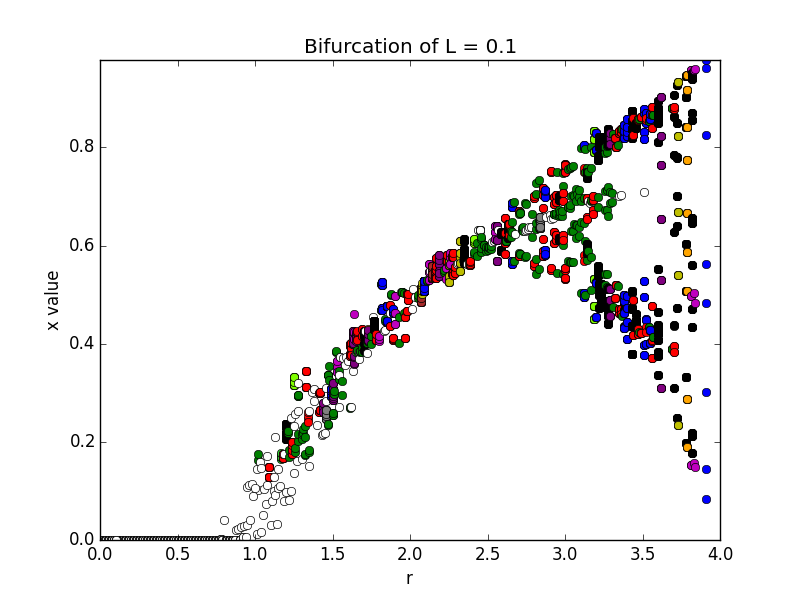
\includegraphics[scale=0.5]{Bifurcation_L1}
\caption{Bifurcation with $L=0.1$}
	\end{center}
\end{figure}
\begin{figure}[H]
	\begin{center}
		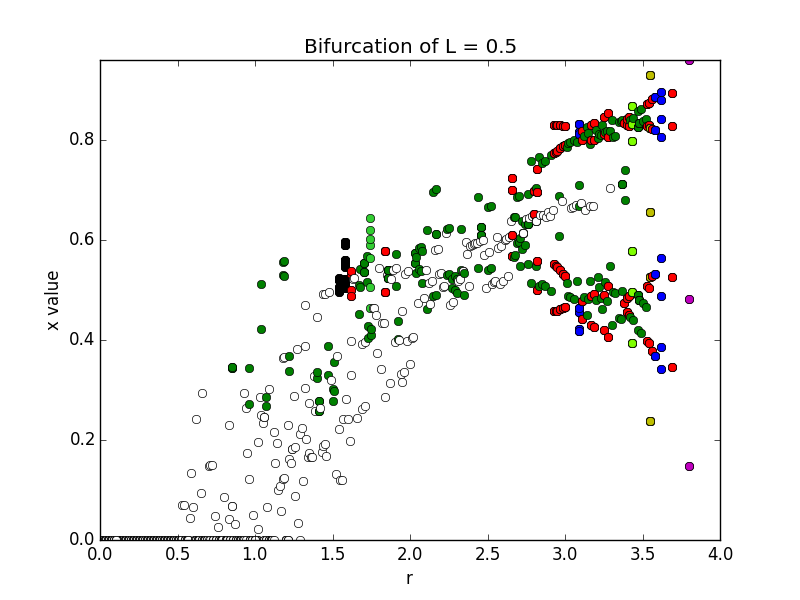
\includegraphics[scale=0.5]{Bifurcation_L5}
\caption{Bifurcation with $L=0.1$}
	\end{center}
\end{figure}

\section{Conclusion}


% \begin{figure}[H]
% 	\begin{center}
% 		\includegraphics[scale=0.7]{deterministic}
% \caption{The deterministic Logistic Map.}
% 	\end{center}
% \end{figure}

\bibliographystyle{plain}
\bibliography{annot}

\end{document}
